\section{Background}
\label{sec:background}

\subsection{Conv2D tensor operation}
A convolutional layer aims to learn feature representations from an input layer. The convolution layer is made of convolution kernels that are used to compute feature maps. Each unit of a feature map is connected to a region of neighboring units of the input maps (the previous layer). Such a neighborhood of the previous layer is known as the receptive field of the unit. A new feature map can be obtained by first convolving the input maps with a learned kernel and then applying a nonlinear elementwise activation function to the convolved results. All spatial locations in the input maps share a kernel to generate a feature map. All feature maps are obtained by convolving several different kernels\cite{gu2018recent}.


The 2D convolution process is performed by the \emph{Conv2D} tensor operation, described in \Equ{eq:conv2D}, where $h$ is the input feature maps, $W$ is the convolution kernels (known as filters), and $b$ is the bias for the output feature maps\cite{goodfellow2016deep}. We denote \emph{Conv} as \emph{Conv2D} operator.
\begin{eqnarray} \label{eq:conv2D}
Conv\left(W,h\right)_{i,j,o}=\sum_{k,l,m}^{K,L,M} h_{(i+k,j+l,m)} W_{(o,k,l,m)}+b_{o}
\end{eqnarray}

\subsection{Floating-point Number Representation}
The representation of every numerical value, in any number system, is made of an integer and a fractional part. The border that delimits them is called the radix point. The fixed-point format for representing numeric values derives its name from the fact that in this format, the base point is fixed at a certain position. For integer numbers, this position is at the right of the least significant digit.

In scientific computation, it is often necessary to represent very large and very small values. This is difficult to achieve using the fixed point format because the bit size/width required to maintain both the desired precision and the desired range are very large. In such situations, floating-point formats are used to represent real numbers. Each floating-point number can be divided into three fields: sign $S$, exponent $E$, and mantissa $M$. Using the binary number system, it is possible to represent any floating-point number as:

\begin{eqnarray} \label{eq:float}
(-1)^{S} \times 1.M \times 2^{E-B}
\end{eqnarray}

In this representation the exponent is biased, this means that the stored value is offset from 0 by a given value depending on the bit size of the exponent field in the particular format. This exponent bias is defined by \Equ{eq:float_bias}, where $E_{size}$ is the exponent bit size.

\begin{eqnarray} \label{eq:float_bias}
B=2^{E_{size}-1}-1
\end{eqnarray}

There is a natural trade-off between reduced bit size requiring fewer hardware resources and larger bit size providing higher precision. Within a given total bit size, it is possible to assign various combinations of bit widths to the exponent and mantissa fields, with wider exponents resulting in a higher range and wider mantissa resulting in better precision.

The most widely used format for floating-point arithmetic is the IEEE 754 standard \cite{zuras2008ieee}. The IEEE single-precision format (32-bit) is expressed in \Equ{eq:float} with $B$ = 127, 8 bits for the exponent and 23 bits for the mantissa, see \Fig{fig:floating}(a). The numbers are normalized, the leading one is an implicit bit, and only the fractional part is explicitly stored in the mantissa field.

\begin{figure}[h!]
	\centering
	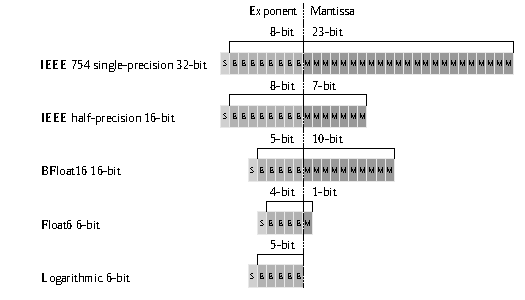
\includegraphics[width=1\columnwidth]{../figures/power_breakdown/floating_point.pdf}
	\caption{Floating-point number representation.}
	\label{fig:floating}
\end{figure}

Reduced bit size than those specified in the IEEE 754 standard are often sufficient to provide the desired precision. Reduced bit size designs require fewer hardware resources enabling low-power implementations. In custom hardware designs, it is possible to customize the exact floating-point format implemented. In later sections, we use the term E$a$M$b$ to denote floating-point representations, where $a$ and $b$ are the exponent and mantissa bit size, respectively. For example, E4M1 means 4-bit exponent and 1-bit mantissa, see \Fig{fig:floating}(d).